%% ============================================================
%%  CHAPITRE 1 — Contexte, Problématique et Étude de l'Existant
%% ============================================================

\section*{Introduction}

Ce chapitre pose les fondements du projet en présentant le contexte dans lequel il s'inscrit,
la problématique identifiée en début de stage, ainsi qu'une analyse rigoureuse de l'existant.
L'objectif est de justifier la nécessité d'une transformation profonde des pratiques de
développement et de livraison logicielle, en s'appuyant sur des données concrètes et une
comparaison avec les standards industriels actuels.


\section{Présentation de l'Organisme d'Accueil}

Sopra HR Software est une Société de Services et d'Ingénierie Informatique (SSII), filiale de
Sopra Steria.

Dans cette section, nous présentons d'abord Sopra Steria, puis Sopra HR Software, et
enfin le département d'accueil au sein duquel ce stage a été réalisé.

\subsection{Sopra Steria}

Sopra Steria est un acteur majeur de la transformation numérique sur le marché européen.
Le groupe propose un portefeuille complet de services couvrant le conseil, l'intégration de
systèmes, l'édition de solutions métiers, la gestion des infrastructures et les services de
processus métier. Ce portefeuille répond aux enjeux de développement et de compétitivité
des grandes entreprises.

La valeur ajoutée de Sopra Steria réside dans sa capacité à accompagner ses clients tout au
long de leur transformation, en combinant innovation et performance opérationnelle.

Le groupe aide ses clients à tirer parti du numérique grâce à des logiciels métiers dans les
domaines de la banque, des ressources humaines (notamment Pleiades et HR Access), ainsi
que de la gestion immobilière (Ulis, Ikos et Altaix).

Le groupe Sopra Steria a enregistré un chiffre d'affaires de 3,8 milliards d'euros en 2017,
avec plus de 42 000 collaborateurs dans plus de 20 pays [1].

\subsection{Sopra HR Software}

Sopra HR Software est une filiale de Sopra Steria spécialisée dans la gestion des ressources
humaines, la paie et la gestion des talents aux niveaux national et international.

Sopra HR propose des solutions RH adaptées aux besoins des directions des ressources
humaines des grandes et moyennes organisations, dans les secteurs public et privé.

Sopra HR est présent dans 10 pays, dont l'Allemagne, la Belgique, le Luxembourg, l'Italie,
la Suisse, le Royaume-Uni, la Tunisie, le Maroc et l'Espagne, garantissant une proximité
géographique et des services adaptés aux besoins des clients [2].

\begin{figure}[h]
    \centering
    \fbox{\parbox{0.82\textwidth}{\centering Espace réservé pour la Figure 1.1\\Vue globale de Sopra HR}}
    \caption{Vue globale de Sopra HR}
    \label{fig:sopra_hr_global_overview}
\end{figure}

\subsection{Département d'Accueil}

Afin d'assurer le bon déroulement des activités et de garantir un haut niveau de service,
plusieurs départements collaborent au sein de Sopra HR.

\begin{figure}[h]
    \centering
    \fbox{\parbox{0.82\textwidth}{\centering Espace réservé pour la Figure 1.2\\Organigramme de Sopra HR Software}}
    \caption{Organigramme de Sopra HR Software}
    \label{fig:sopra_hr_org_chart}
\end{figure}

Notre stage de fin d'études a été réalisé au sein de l'\textbf{équipe QA (Quality Assurance)
internationale}. Cette équipe a pour mission de garantir la qualité des livrables logiciels
produits par les équipes de développement, en concevant et en exécutant des campagnes de tests
automatisés sur les solutions RH de Sopra HR (notamment HR Access et Pleiades).

L'équipe QA s'appuie sur un framework interne de tests BDD (\textit{Behavior-Driven
Development}) nommé \textbf{T4T} (\textit{Test for Teams}). Ce framework permet aux testeurs
de rédiger des scénarios de test en langage naturel structuré (syntaxe Gherkin~:
\texttt{Given/When/Then}) qui sont ensuite exécutés automatiquement contre les applications
cibles. T4T est l'outil central de la stratégie de test de l'équipe.

\begin{figure}[H]
    \centering
    \fbox{\parbox{0.85\textwidth}{\centering
        \vspace{2.5cm}
        Espace réservé pour la Figure~\ref{fig:t4t_overview}\\
        \textbf{Vue d'ensemble du framework T4T et son intégration dans le workflow QA}\\[6pt]
        \footnotesize Scénarios BDD (Gherkin) $\to$ T4T Engine $\to$ Exécution $\to$ Rapports
        \vspace{2.5cm}
    }}
    \caption{Framework T4T~: vue d'ensemble du workflow de tests BDD}
    \label{fig:t4t_overview}
\end{figure}


\section{La Mission~: Du Jenkins Basique à une Chaîne DevSecOps}

Dans ce contexte d'équipe QA, la mission confiée pour ce projet de fin d'études est
précisément définie en trois volets~:

\begin{enumerate}
    \item \textbf{Concevoir de nouveaux pipelines CI/CD}~: remplacer l'approche Jenkins
    vieillissante par des pipelines modernes, automatisés et maintenables avec GitHub Actions~;
    \item \textbf{Sécuriser la chaîne de livraison}~: intégrer des contrôles de sécurité
    (SAST, SCA, DAST) à chaque étape du pipeline, selon le principe DevSecOps Shift-Left~;
    \item \textbf{Générer des rapports d'analyse automatisés}~: chaque exécution du pipeline
    doit produire des rapports de tests, de couverture, de vulnérabilités et de conformité,
    auditables et archivés comme artefacts.
\end{enumerate}

Pour mener à bien cette mission, une \textbf{application web de démonstration} (Todo App
React) a été développée comme support concret. Cette application permet de valider
l'ensemble de la chaîne DevSecOps dans un contexte réaliste~: tests unitaires, tests E2E,
scans de sécurité, déploiement sur Kubernetes, et monitoring --- le tout applicable ensuite
aux projets réels de l'équipe QA utilisant T4T.


\section{Le Modèle <<Deploy First, Secure Later>> et ses Limites}

Pendant longtemps, les équipes de développement ont fonctionné selon un modèle où la sécurité
était traitée comme une \textbf{étape finale}, voire optionnelle. On codait, on testait les
fonctionnalités, on déployait et on pensait à la sécurité <<plus tard>>, souvent lors
d'un audit annuel ou après un incident.

Ce modèle présente des problèmes fondamentaux résumés dans le tableau \ref{tab:deploy_first} :

\begin{table}[h]
    \centering
    \setlength{\arrayrulewidth}{0.8pt}
    \setlength{\dashlinedash}{3pt}
    \setlength{\dashlinegap}{2pt}
    \renewcommand{\arraystretch}{1.4}
    \caption{Problèmes du modèle <<Deploy First, Secure Later>>}
    \label{tab:deploy_first}
    \begin{tabularx}{\textwidth}{|>{\centering\arraybackslash}X|>{\centering\arraybackslash}X|}
\hline
\tableheader \textbf{Problème} & \textbf{Conséquence} \\
\hline
Vulnérabilités découvertes tard dans le cycle & Coût de correction 10x à 100x plus élevé \\ \hdashline
Secrets hardcodés dans le code & Risque de compromission de l'infrastructure \\ \hdashline
Images Docker non scannées & CVEs critiques en production \\ \hdashline
Accès réseau non restreints & Propagation latérale en cas d'intrusion \\ \hdashline
Pas de monitoring sécurité runtime & Détection des attaques impossible \\
\hline
    \end{tabularx}
\end{table}


\section{Les Pressions Réglementaires et Industrielles}

En 2026, les exigences réglementaires renforcent la nécessité d'une sécurité intégrée:

\begin{itemize}
    \item \textbf{NIS2} (\textit{Network and Information Security Directive}) impose des contrôles
    de sécurité sur les chaînes d'approvisionnement logicielles;
    \item \textbf{DORA} (\textit{Digital Operational Resilience Act}) impose la résilience et
    la traçabilité des changements;
    \item \textbf{ISO 27001} et \textbf{SOC 2} sont devenus des critères de sélection des
    fournisseurs de services numériques;
    \item Les standards \textbf{SLSA} (\textit{Supply-chain Levels for Software Artifacts})
    définissent des niveaux d'intégrité des artefacts logiciels.
\end{itemize}


\section{Problématique Centrale}

La problématique de ce projet se formule ainsi:

\begin{infobox}
    \textit{Comment concevoir de nouveaux pipelines CI/CD pour remplacer l'approche Jenkins
    existante de l'équipe QA, en intégrant la sécurité à chaque étape selon une approche
    DevSecOps, tout en produisant des rapports d'analyse automatisés et auditables, sans
    sacrifier la vélocité de livraison~?}
\end{infobox}

Cette problématique est multidimensionnelle:
\begin{itemize}
    \item \textbf{Technique:} Quels outils choisir? Comment les intégrer?
    \item \textbf{Organisationnelle:} Comment \textit{shift-left} la sécurité dans les pratiques
    d'équipe?
    \item \textbf{Économique:} Comment démontrer le ROI de la sécurité intégrée?
    \item \textbf{Opérationnelle:} Comment maintenir la visibilité sur un système distribué
    complexe?
\end{itemize}


\section{Étude de l'Existant --- L'Approche Jenkins}

\subsection{Description de l'Ancienne Architecture}

Avant ce projet, le système en place reposait sur une approche minimaliste et très courante
dans les petites équipes~: un serveur Jenkins auto-hébergé configuré et maintenu de manière
manuelle.

L'équipe QA exécutait ses \textbf{tests BDD} rédigés avec le framework interne
\textbf{T4T} via des jobs Jenkins. Ces tests, écrits en syntaxe Gherkin
(\texttt{Given/When/Then}), validaient les scénarios fonctionnels des applications RH.
Cependant, les jobs Jenkins étaient définis et administrés à la main par les développeurs, et
les builds étaient souvent lancés manuellement plutôt que par des déclencheurs automatisés.
Jenkins était relié au dépôt Git, mais l'intégration restait limitée~: il se contentait
d'exécuter les tests BDD T4T avant un déploiement manuel effectué via des scripts shell.
\textbf{Aucun contrôle de sécurité} n'était intégré dans ce pipeline.

La figure \ref{fig:jenkins_architecture_existant} présente l'architecture logique de cette
approche Jenkins avant la transformation DevSecOps.

\begin{figure}[H]
    \centering
    % Simple image include (provide images/old_jenkins_logical_architecture.(pdf|png|jpg) in the images/ folder)
    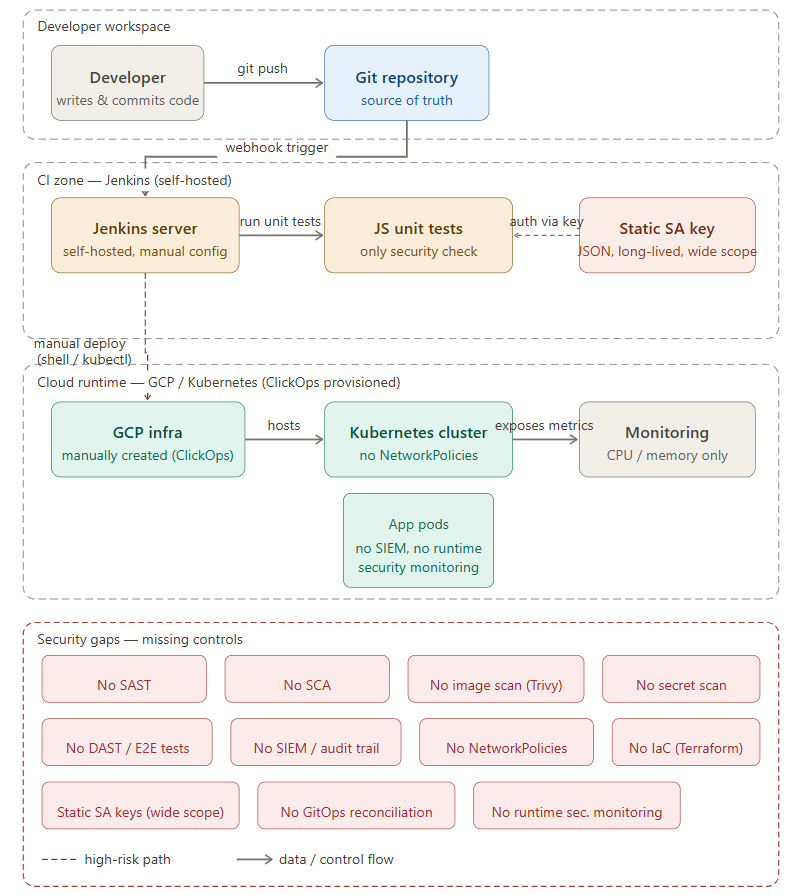
\includegraphics[width=0.9\textwidth,keepaspectratio]{images/old_jenkins_logical_architecture}
    \caption{Architecture logique de l'approche Jenkins (état initial)}
    \label{fig:jenkins_architecture_existant}
\end{figure}

Le tableau \ref{tab:etat_avant} synthétise l'état de l'art avant la transformation:

\begin{table}[h]
    \centering
    \setlength{\arrayrulewidth}{0.8pt}
    \setlength{\dashlinedash}{3pt}
    \setlength{\dashlinegap}{2pt}
    \renewcommand{\arraystretch}{1.4}
    \caption{État du système avant la transformation DevSecOps}
    \label{tab:etat_avant}
    \begin{tabularx}{\textwidth}{|>{\centering\arraybackslash}X|>{\centering\arraybackslash}X|}
\hline
\tableheader \textbf{Aspect} & \textbf{État Avant} \\
\hline
Outil CI & Jenkins (auto-hébergé, configuration manuelle) \\ \hdashline
Tests & Tests BDD uniquement (framework T4T interne) \\ \hdashline
Sécurité & \textbf{Aucune} \\ \hdashline
Scan de vulnérabilités & Absent \\ \hdashline
Scan des images Docker & Absent \\ \hdashline
Scan des secrets & Absent \\ \hdashline
Tests E2E & Absents ou manuels \\ \hdashline
Infrastructure & Créée manuellement via console GCP (ClickOps) \\ \hdashline
Déploiement & Scripts shell ad-hoc, pas versionnés \\ \hdashline
Authentification CI & Clés JSON longue durée dans les secrets Jenkins \\ \hdashline
Monitoring & Basique (CPU/mémoire uniquement) \\ \hdashline
Sécurité réseau & Pas de NetworkPolicies \\ \hdashline
SIEM & Absent \\ \hdashline
Audit trail & Inexistant \\
\hline
    \end{tabularx}
\end{table}

\subsection{Problèmes Identifiés}

\textbf{Problème 1 --- Absence totale de sécurité dans le pipeline:}
Le pipeline Jenkins se contentait de vérifier que les tests BDD T4T passaient. Aucune analyse
statique de sécurité (SAST), aucun scan de dépendances (SCA), aucun scan d'images Docker
n'était effectué. Des vulnérabilités critiques pouvaient transiter du code source jusqu'en
production sans être détectées.

\textbf{Problème 2 --- Clés d'authentification statiques:}
Jenkins utilisait des clés JSON Google Cloud Service Account avec des permissions larges, stockées
en clair dans la configuration Jenkins. La compromission de ces clés aurait donné un accès complet
à l'infrastructure GCP.

\textbf{Problème 3 --- Infrastructure non reproductible:}
Les ressources GCP (cluster Kubernetes, réseau, IAM) étaient créées manuellement via la console.
Il était impossible de recréer l'environnement de façon fiable, et les modifications n'étaient
pas tracées.

\textbf{Problème 4 --- Déploiements impératifs non versionnés:}
Les déploiements étaient effectués via des commandes \texttt{kubectl apply} ou des scripts shell
non versionnés, sans historique, sans rollback automatique et sans validation de l'état désiré.

\textbf{Problème 5 --- Aucune visibilité sur la sécurité en production:}
Après le déploiement, aucun outil ne surveillait les comportements anormaux, les tentatives
d'intrusion ou les événements de sécurité sur les nœuds Kubernetes.

\textbf{Problème 6 --- Tests non représentatifs:}
Les tests BDD T4T ne couvraient que les scénarios fonctionnels métier, sans jamais valider
le comportement réel de l'application dans son contexte de déploiement cloud-native.
Aucun test de sécurité, aucun test E2E dans le cluster, et aucun scan dynamique n'étaient
réalisés. De plus, aucun rapport d'analyse de sécurité n'était généré.

\subsection{Dette Technique et Sécuritaire Accumulée}

 Le tableau \ref{tab:owasp_avant} résume la dette accumulée selon les catégories OWASP Top 10:

\begin{table}[h]
    \centering
    \setlength{\arrayrulewidth}{0.8pt}
    \setlength{\dashlinedash}{3pt}
    \setlength{\dashlinegap}{2pt}
    \renewcommand{\arraystretch}{1.4}
    \caption{Couverture OWASP Top 10 avant ce projet}
    \label{tab:owasp_avant}
    \begin{tabularx}{\textwidth}{|>{\centering\arraybackslash}X|>{\centering\arraybackslash}X|}
\hline
\tableheader \textbf{Catégorie OWASP} & \textbf{État Avant} \\
\hline
A01 - Broken Access Control & Non contrôlé (credentials hardcodés) \\ \hdashline
A02 - Cryptographic Failures & Secrets en clair dans le code et CI \\ \hdashline
A03 - Injection (XSS) & Non détecté, pas de SAST \\ \hdashline
A05 - Security Misconfiguration & Containers root, pas de NetworkPolicies \\ \hdashline
A06 - Vulnerable Components & Dépendances jamais auditées \\ \hdashline
A08 - Software Integrity Failures & Images non signées, pas de SBOM \\ \hdashline
A09 - Security Logging Failures & Aucun SIEM, aucun audit trail \\
\hline
    \end{tabularx}
\end{table}


\section*{Conclusion}

Ce chapitre a établi le contexte général du projet en identifiant les six lacunes majeures de
l'approche Jenkins initiale et en formulant la problématique centrale~: intégrer la sécurité
à chaque étape du cycle de livraison sans sacrifier la vélocité.
L'analyse de la dette technique
et sécuritaire accumulée, notamment au regard du référentiel OWASP Top 10, justifie pleinement
l'ampleur de la transformation entreprise.
Le chapitre suivant présente l'analyse des besoins
fonctionnels et non fonctionnels identifiés pour répondre à cette problématique.

